Let us now consider a $N$-body problem, with $N>2$ gravitationally interacting
objects. We will solve this system with the \textit{direct summation method}.
First, however, let us cast the problem in dimensionless units. The $N$-body
equation reads
\begin{align}
    \frac{d\vec{x}_i}{dt}
    &=\vec{v}_i \\
    m_i\frac{d\vec{v}_i}{dt}
    &=Gm_i\sum_{k\neq i}m_k\frac{\vec{x}_k-\vec{x}_i}{|\vec{x}_k-\vec{x}_i|^3}
\end{align}

\subsection{Show that with an appropriate scaling $\vec x=\xi\vec x'$,
    $\vec v=\Phi\vec v'$, $t=\tau t'$ and $m=\mu m'$ (with $\xi,\Phi,\tau$
    and $\mu$ constants) the equations for $N$-body dynamics can be brought 
    into dimensionless form, where the gravitational constant $G$ is absorbed
    into the variables. Which condistions must $\xi,\Phi,\tau$ and $\mu$ obey
    and how many of them can be freely chosen?
}
    % \begin{itemize}
    %     \item chain rule $\Rightarrow\phi=\xi/\tau$
    % \end{itemize}
    Dimensionless quantities must fulfill:
    \begin{align}
        \tder{\vec{x_i}'}{t'}
        &= \vec{v_i'} 
        \label{eq:wdim1} \\
        m_i' \tder{\vec{v_i'}}{t'}
        &= m_i' \sum_{k\neq i} m_k'
        \frac{\vec{x_k}' -\vec{x_i}'}{|\vec{x_k}'-\vec{x_i}'|^3}
 	\label{eq:wdim2}   
    \end{align}
    From \autoref{eq:wdim1} we can calculate 
    \begin{align}
        \tder{\vec{x_i}'}{t'}&\overset{CR}{=} 
        \frac{\tau}{\xi} \tder{\vec{x}}{t}
        \overset{!}{=}\vec{v_i}' 
        =\frac{\vec{v_i}}{\phi} \\
        \Rightarrow\phi&=\frac{\xi}{\tau}
    \end{align}
    Since $[G] = \frac{\text{m}^3}{\text{kg } \text{s}^2}$, we can 
    couple $\mu$, $\tau$ and $\xi$. Together we have 4 unknowns and two 
    constraints, therefore we can choose two paratemer freely.
    We choose: $\mu = M_*$ und $\xi=1$ AU. 
    It follows that 
    $\tau=\sqrt{\frac{\xi^3}{G \mu}}\approx 5.02\cdot 10^6\text{s} 
    \approx 58.1 \text{d}$ 
    and $\phi=\sqrt{\frac{G \mu}{\xi}}\approx3\cdot10^4
    \frac{\text{m}}{\text{s}}$. \\
    \\
    From now on we will do everything in these dimensionless units.

\newpage
\subsection{Write an $N$-body code for arbitrary $N$ with the leapfrog 
    integration and a constant time step.
} 
    One way to prevent numerical divergences in case of very close encounters 
    is to use the \textit{softening length parameter} $\varepsilon$ and modify 
    the gravitational force among massive particles:
    \begin{equation}
        m_i\frac{d\vec v_i}{dt}
        =Gm_i\sum_{k\neq i}m_k\frac{\vec x_k-\vec x_i}
        {|\vec x_k-\vec x_i|^3 + \varepsilon^3}
    \end{equation}
    However, $\varepsilon$ should be small enough to keep the simulation 
    physically consistent. We set:
    \begin{equation}
        \varepsilon=LN^{-1/3}\cdot\frac{1}{10000},
    \end{equation}
    where $L$ is the typical size of the system in dimensionless units and 
    $N$ is the number of particles. \\
    \\
    We can implement this directly when defining a class holding all of the 
    information about a planet:
    \begin{lstlisting}
        class Planet():
            def __init__(self, r_0, v_0, m):
                self.r = r_0
                self.v = v_0
                self.m = m
                self.trajectory = []
                self.velocities = []
        
            def update_velocity(self, planets, dt):
                for p in planets:
                    if p == self:
                        continue
                    epsilon = 2 * len(planets)**(-1/3) / 10000
                    delta_r = p.r - self.r
                    a = G * p.m * delta_r / (norm(delta_r)**3 + epsilon**3)
                    self.v = np.add(self.v, a * dt)
        
                self.velocities.append(self.v)
        
            def update_position(self, dt):
                self.r = np.add(self.r, self.v * dt)
                self.trajectory.append(self.r) \end{lstlisting}

    \paragraph{As a simple test problem, solve the following sample binary 
        star problem: two stars of mass $1$ at initial locations 
        $\vec x_1=(-0.5,0,0)$, $\vec x_2=(+0.5,0,0)$ and initial velocities
        $\vec v_1=(0,-0.5,0)$, $\vec v_2=(0,+0.5,0)$. Choose an appropriate
        time step! Plot the resulting trajectories of both starts in the 
        $(x,y)$-plane (projection). Plot also the time evolution of the 
        relative error of the total energy of the system.
    } \ \\
        \\
        \begin{figure}[h!]
            \centering
            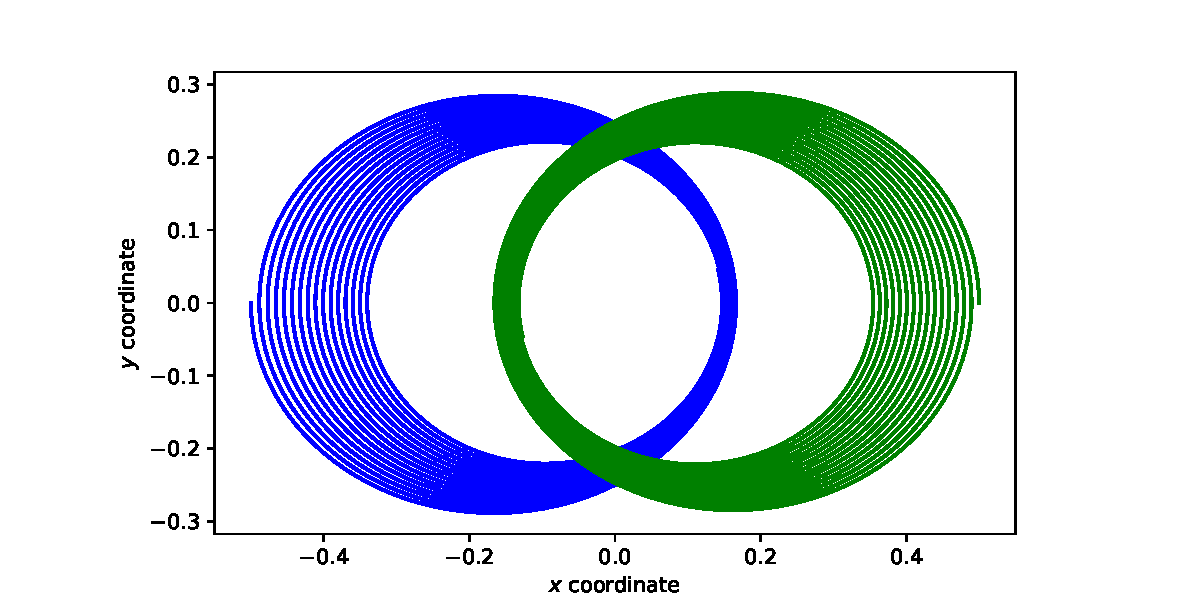
\includegraphics[width=\textwidth]{./figures/task2_2body.pdf}
            \caption{}
        \end{figure} \ \\ 

    \newpage
    \paragraph{Now add a third star with mass $0.1$ and initial position 
        $\vec x_3=(1,6,2)$ and initial velocity $\vec v_3=(0,0,0)$. Show how 
        this third star "falls into" the binary, interacts with it, and gets 
        eventually ejected. Plot the trajectories of all three stars in the 
        $(x,y)$-plane (projection). Again, plot the time evolution of the 
        relative error of the total energy of the system.
    } \ \\
        \\
        \begin{figure}[h!]
            \centering
            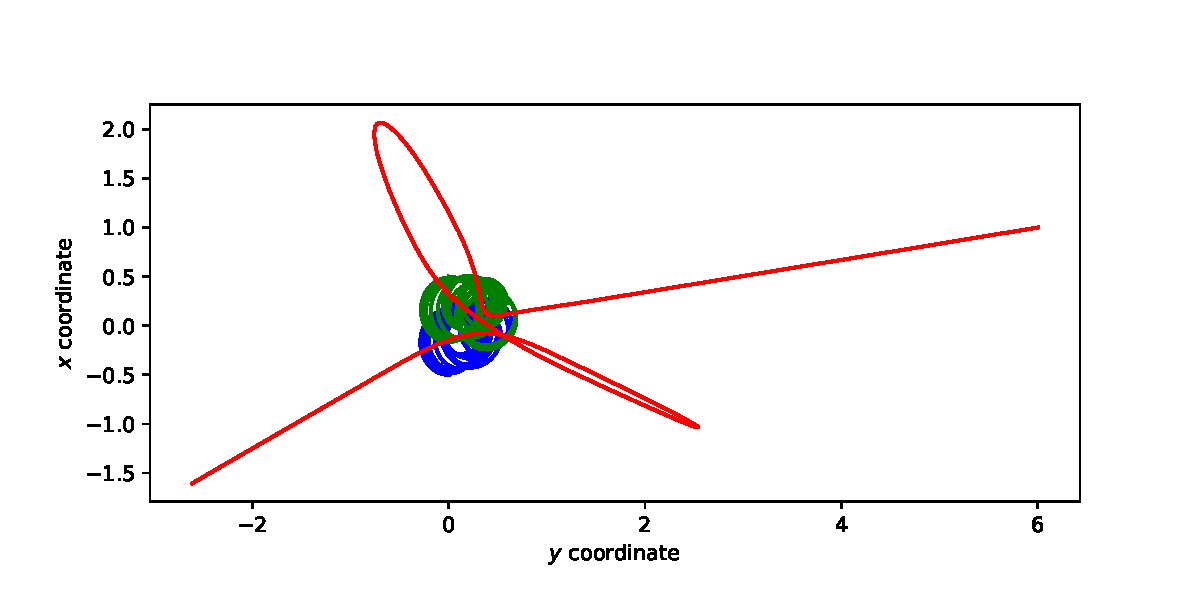
\includegraphics[width=\textwidth]{./figures/task2_3body.pdf}
        \end{figure} \ \\ 
        \begin{figure}[h!]
            \centering
            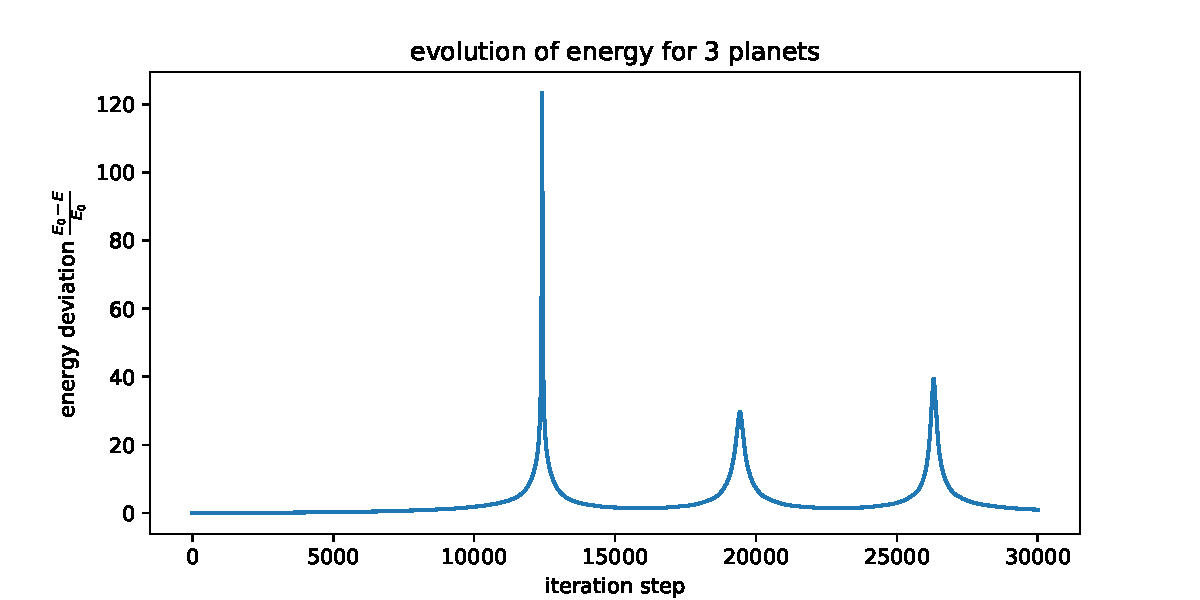
\includegraphics[width=\textwidth]{./figures/task2_3body_energy_new.pdf}
        \end{figure} \ \\ 
    
    \paragraph{Play with the time step by varying it at least a factor of 10 
        (but keep the final time of the integration fixed) and describe whether 
        the results change or not. The effect of changing the time step can 
        also be stronger than in this case, to see this also try 
        $\vec x_3=(1,6,3)$
    } \ \\
        \\
        \begin{itemize}
            \item overall behavior is similar: star falls in, gets 
                "thrown around", then ejected
            \item details are different, e.g. direction of ejection
        \end{itemize}

\newpage
\subsection{Real $N$-body problem ($N>>3$)}
    \paragraph{Set up a spherical cloud of 30 randomly positioned stars of 
        mass 1. The cloud radius is 1. Use a uniform random number generator 
        for this. An easy way is to choose randomly $(x,y,z)$ between 
        $-1$ and $+1$, and reject (and redo) stars that have 
        $1<\sqrt{x^2+y^2+z^2}$. Give each particle a random velocity
        (uniform) with a maximum of $0.1$. Use the same rejection trick as for 
        the positions. Evolve the system over an appropriate time-scale 
        (is there a characteristic time-scale for gravitationally interacting
        cluster?). 
    } \ \\
        \\
        A system of 30 randomly-distributed planets (in a sphere) can 
        be created using the following function:
        \begin{lstlisting}
            def create_30_body_system():
                planets = []
                for _ in range(30):
                    valid_r, valid_v = False, False
                    while not valid_r:
                        x = uniform(-1, 1)
                        y = uniform(-1, 1)
                        z = uniform(-1, 1)
                        if np.sqrt(x**2 + y**2 + z**2) <= 1:
                            valid_r = True
                    while not valid_v:
                        vx = uniform(-.1, .1)
                        vy = uniform(-.1, .1)
                        vz = uniform(-.1, .1)
                        if np.sqrt(vx**2 + vy**2 + vz**2) <= .1:
                            valid_v = True
            
                    r, v, m = np.array([x, y, z]), np.array([vx, vy, vz]), 1
                    p = Planet(r, v, m)
            
                    planets.append(p)
            
                return planets \end{lstlisting} \ \\
        For the following simulations, we will have to use an adaptive 
        time-step: at the beginning of each iteration, we estimate the 
        value of the time-step as 
        \begin{equation}
            \Delta t = C\cdot\frac{d_{min}}{|\vec v_{max}|},
        \end{equation}
        where $C=0.01$. $d_{min}$ is the minimum distance between 2 particles 
        and $|\vec v_{max}|$ is the velocity of the fastest particle in the 
        system. If the evolution is unstable or if the relative error of the 
        total energy gets higher than 0.05, decrease the value of $C$ (note 
        that in this case you will need more iteration steps to evolve the 
        system to the same time scale).

        \newpage \noindent
        To implement this, at each time step we run the following function:
        \begin{lstlisting}
            def calculate_adaptive_dt(planets):
                ds, vs = [], []
                for p in planets:
                    for q in planets:
                        if p is q:
                            continue
                        ds.append(norm(p.r - q.r))
                    vs.append(norm(p.v))
                d_min = min(ds)
                v_max = max(vs)
                return 0.1 * d_min / v_max \end{lstlisting} \ \\
        % \begin{figure}[h!]
        %     \centering
        %     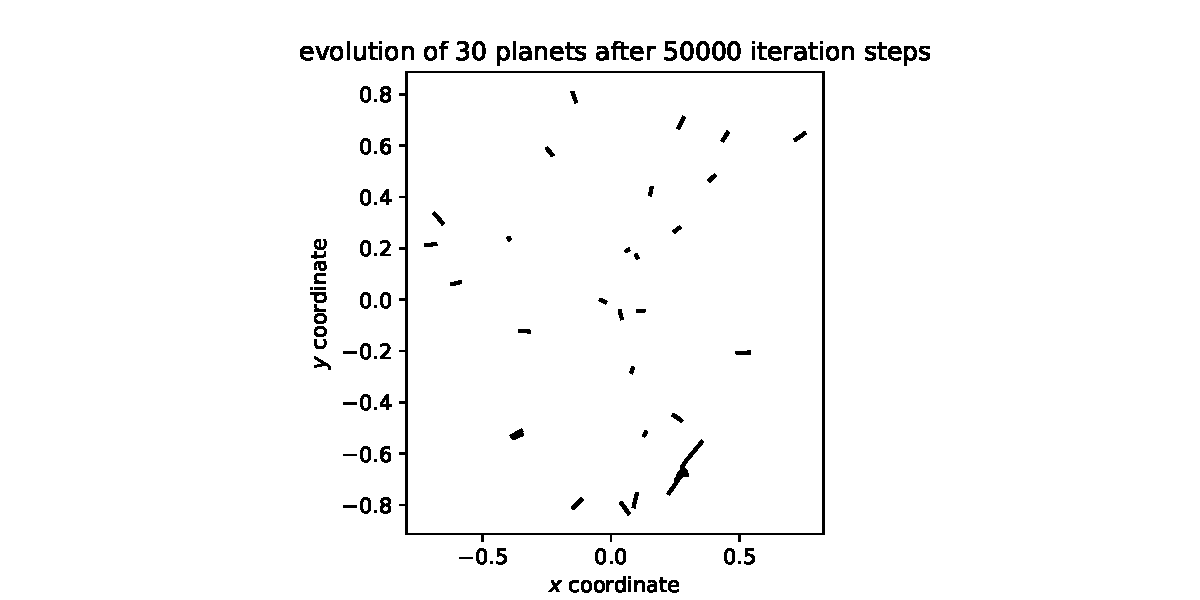
\includegraphics[width=\textwidth]{./figures/task2_30body.pdf}
        % \end{figure} \ \\ 
        We choose $C=1$ for reasons of computation time.


    \paragraph{Plot the time evolution of the relative error of the total 
        energy.
    } \ \\
        \\ 
        The simulation is run for $50000$ iterations:
        \begin{figure}[h!]
            \centering
            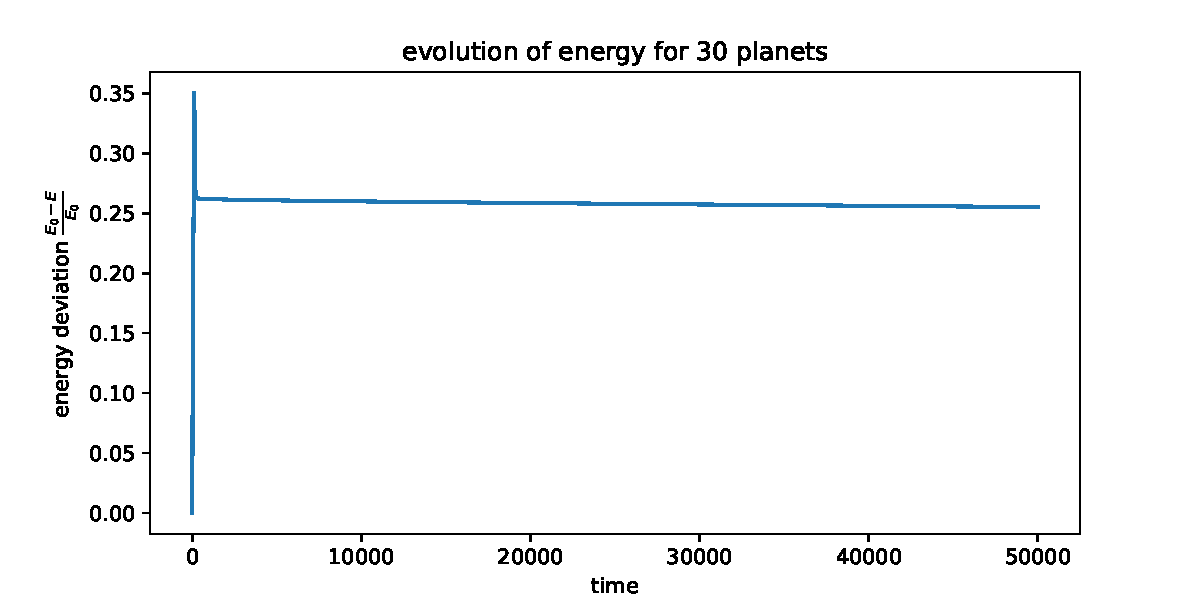
\includegraphics[width=\textwidth]{./figures/task2_30body_energy_new.pdf}
        \end{figure} \ \\ 

    \newpage
    \paragraph{Plot the evolution in 3D and note any interesting patterns that 
        emerge from the evolution. What are these? Why do they appear?
    } \ \\
        \\
        ...
        \begin{figure}[h!]
            \centering
            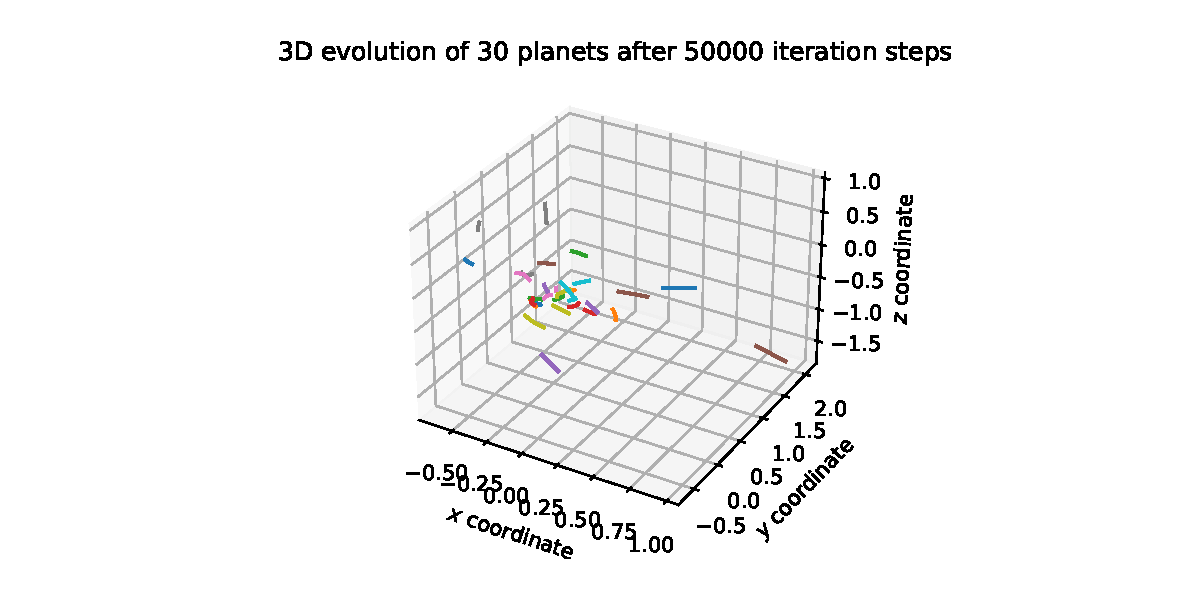
\includegraphics[width=\textwidth]{./figures/task2_30body_3D_new.pdf}
        \end{figure} \ \\ 

    \paragraph{Now redo the simulation with $N=60$ and masses $m=0.5$. Run this and 
        the previous simulation for 100 iterations each. Compare both the 
        results and run times between the two.
    } \ \\
        \\
        ...
